\newcommand{\chapter}[2][]{
	\newcommand{\chapname}{#2}
	\begin{flushleft}
		\begin{minipage}[t]{\linewidth}
			
\includegraphics[height=1cm]{hdht-logo.png}
			\hspace{0pt}	
			\sffamily\bfseries\large Bài 5: Tổng hợp hai dao động điều hòa cùng phương,
			cùng tần số. Phương pháp giản đồ Fre-nen
			\begin{flushleft}
				\huge\bfseries #1
			\end{flushleft}
		\end{minipage}
	\end{flushleft}
	\vspace{1cm}
	\normalfont\normalsize
}
\chapter[Dạng bài: Đồ thị dao động điều hòa]{Dạng bài: Đồ thị dao động điều hòa}
\section{Lý thuyết}
\subsection{Đồ thị dao động cơ}
Xét phương trình dao động điều hoà: $x = A \cos(\omega t+\varphi)$, nếu chọn gốc thời gian và chiều dương trục toạ độ thích hợp để $\varphi = 0$. Ta lập bảng giá trị sau để vẽ đồ thị của hàm điều hoà $x = A \cos(\omega t+\varphi)$:
\begin{center}
	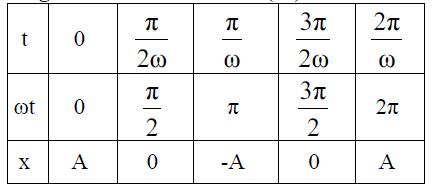
\includegraphics[scale=0.7]{../figs/VN12-PH-06-A-004-2-V2-02.jpg}
\end{center}
\begin{center}
	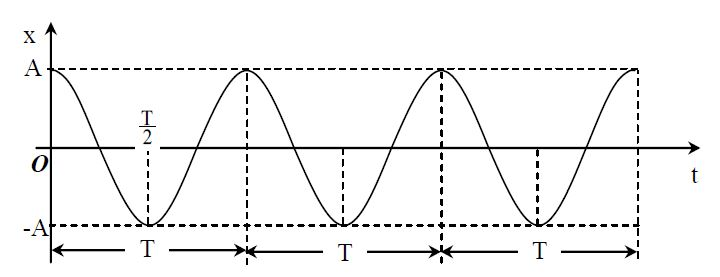
\includegraphics[scale=0.6]{../figs/VN12-PH-06-A-004-2-V2-01.jpg}
\end{center}
\subsection{Đồ thị và sự so sánh pha của các dao động điều hòa: $x$, $v$, $a$.}
Vẽ đồ thị của dao động $x = A \cos(\omega t+\varphi)$ trong trường hợp $\varphi =0$.
\begin{center}
	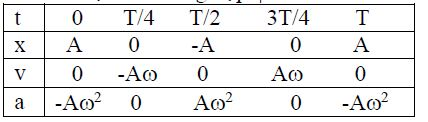
\includegraphics[scale=0.7]{../figs/VN12-PH-06-A-004-2-V2-03.jpg}
\end{center}
\begin{center}
	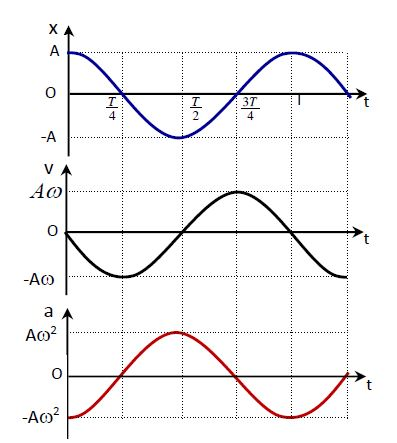
\includegraphics[scale=0.8]{../figs/VN12-PH-06-A-004-2-V2-04.jpg}
\end{center}

\textbf{Nhận xét:}

+ Nếu dịch chuyển đồ thị $v$ về phía chiều dương của trục O$t$ một đoạn thì đồ thị của $v$ và $x$ cùng pha nhau. Nghĩa là, $v$ nhanh pha hơn $x$ một góc $\dfrac{\pi}{2}$ hay về thời gian là $\dfrac{T}{4}$.

+ Nếu dịch chuyển đồ thị $a$ về phía chiều dương của trục O$t$ một đoạn thì đồ thị của $a$ và $v$ cùng pha nhau.

Nghĩa là, $a$ nhanh pha hơn $v$ một góc $\dfrac{\pi}{2}$ hay về thời gian là $\dfrac{T}{4}$.

+ Nhận thấy $a$ và $x$ luôn ngược pha nhau (trái dấu nhau).
\section{Mục tiêu bài học - Ví dụ minh họa}
\begin{dang}{Giải bài tập đồ thị dao động điều hòa}
	\viduii{3}{Hai con lắc lò xo giống nhau đều có khối lượng vật nhỏ là $m$. Lấy mốc thế năng tại vị trí cân bằng và $\pi ^2 = 10$. Gọi $x_1$, $x_2$ lần lượt là li độ dao động của con lắc thứ nhất và thứ hai. Tại thời điểm $t$, con lắc thứ nhất có động năng $0,06\ \text J$ và con lắc thứ hai có thế năng $0,005\ \text J$. Giá trị của $m$ là
		\begin{center}
			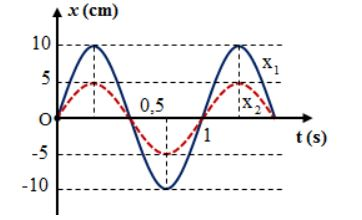
\includegraphics[scale=0.8]{../figs/VN12-PH-06-A-004-2-V2-05.jpg}
		\end{center}
		\begin{mcq}(4)
			\item $100\ \text g$.
			\item $200\ \text g$.
			\item $400\ \text g$.
			\item $800\ \text g$.
		\end{mcq}
	}
	{
		\begin{center}
			\textbf{Hướng dẫn giải}
		\end{center}
		
		Ta có $\omega_1 = \omega_2 = 2 \pi\ \text{rad}$ nên:
		
		$$\dfrac{x_1}{x_2}=\dfrac{A_1}{A_2} \Rightarrow \dfrac{\dfrac{1}{2}kx_1^2}{\dfrac{1}{2}kx_2^2}=\dfrac{A_1^2}{A_2^2}=4 \Rightarrow \dfrac{W_1 - 0,06}{0,005}=4 \Rightarrow W_1 = 0,08\ \text J.$$
		
		Vậy $m=\dfrac{2W_1}{\omega ^2 A_1 ^2} = 400\ \text g$.
		
		
		\textbf{Đáp án: C}.
	}
	
	\viduii{4}
	{
		Cho ba dao động điều hòa cùng phương cùng tần số, có phương trình lần lượt là $x_1=2a\cos \omega t$, $x_2=A_2\cos \left( \omega t+\varphi_2\right) $, $x_3=a\cos \left( \omega t+\pi\right) $. Gọi $x_{12}=x_1+x_2, \ x_{23}=x_2+x_3$. Biết đồ thị sự phụ thuộc của $x_{12}$ và $x_{23}$ vào thời gian như hình vẽ. Giá trị của $\varphi_2$ là	
		\begin{center}
			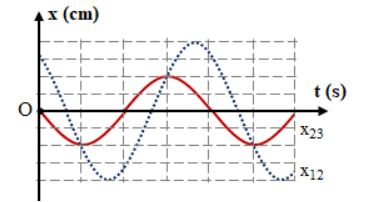
\includegraphics[scale=0.8]{../figs/VN12-PH-06-A-004-2-V2-06.jpg}
		\end{center}	
		\begin{mcq}(4)
			\item $\dfrac{\pi}{3}$.
			\item  $\dfrac{\pi}{4}$.
			\item  $\dfrac{2\pi}{3}$.
			\item  $\dfrac{\pi}{6}$.
		\end{mcq}	
	}{
		\begin{center}
			\textbf{Hướng dẫn giải:}
		\end{center}
		
		Dùng giao điểm $\Rightarrow x_{23}$ sớm pha hơn $\dfrac{\pi}{3}$ so với $x_{12}$.
		
		Đề cho: $x_1+2x_3=0$.
		
		Lại có: $x_{23}=2\angle \dfrac{\pi}{2}=x_2+x_3$ và $x_{12}=4\angle \dfrac{\pi}{6}=x_1+x_2$.
		
		Suy ra $2x_{23}+x_{12}=3x_2\Rightarrow x_2=\dfrac{4\angle \dfrac{\pi}{2}+4\angle \dfrac{\pi}{6}}{3}=\dfrac{4}{\sqrt{3}}\angle \dfrac{\pi}{3}$.
		
		\textbf{Đáp án: A}.
		
	}
	
\end{dang}